\documentclass[12pt,reqno]{amsart}

% --- Packages ---
\usepackage{amsmath,amssymb,amsthm}
\usepackage{mathrsfs}
\usepackage{hyperref}
\usepackage[margin=1in]{geometry}
\usepackage{graphicx}
\usepackage{enumerate}
\usepackage{subcaption} % subtable を使うために必要
\usepackage{booktabs}   % \toprule, \midrule, \bottomrule を使うために必要
\usepackage{xcolor} % 背景色を使うためのパッケージ
\usepackage{placeins}

% --- Theorem Environments ---
\newtheorem{theorem}{Theorem}[section]
\newtheorem{lemma}[theorem]{Lemma}
\newtheorem{corollary}[theorem]{Corollary}
\newtheorem{proposition}[theorem]{Proposition}
\newtheorem{compresult}[theorem]{Computational Result}

\theoremstyle{definition}
\newtheorem{definition}[theorem]{Definition}
\newtheorem{example}{Example}
\newtheorem{conjecture}[theorem]{Conjecture}

\theoremstyle{remark}
\newtheorem{remark}[theorem]{Remark}

\numberwithin{equation}{section}

% --- Title and Author Information ---
% \title[ヘッダー用の短縮タイトル]{表紙・本文用の正式タイトル}
\title[Regularized Prime-Race Statistics]{Regularized Spectral Statistics for Prime Races and Low-Zero Transient Reversals}

\author{Shin-ya Koyama}
\address{Department of Mechanical Engineering, Toyo University, 2100 Kujirai, Kawagoe-shi, 350-8585 Japan}
\email{koyama@toyo.jp}

\author{Saar Shai}
\address{Independent researcher}
\email{saar.shai@gmail.com}

\date{\today}

\begin{document}

\begin{abstract}
We study a proposed Gaussian-regularized statistic for prime races and a
separate finite-scale reconstruction of ordinary prime-count races.  Character
orthogonality gives the exact selector
\[
 \frac1{\varphi(N)}\sum_\chi(1-\overline{\chi(a)})\chi(x)
 =\mathbf 1_{x\equiv1\pmod N}-\mathbf 1_{x\equiv a\pmod N}.
\]
For the regularized statistic we formulate an explicit two-parameter analytic
target with $T=T(x)$; the fixed-$T$ asymptotic is not asserted, because the
diagonal coefficient depends on $T$ and a summed off-diagonal estimate remains
to be proved.  The proposed extremality of $-1\pmod N$ and recessiveness of
$1\pmod N$ are therefore stated as conjectural fine-structure principles.

Independently, we analyze ordinary prime-count data for
$N\in\{7,8,11,19,23\}$ at 438 checkpoints through $3\times10^{14}$.
The extended computation agrees with an independently checked baseline in
567 of 567 shared cells through $1.3\times10^{13}$.  Low-zero explicit-formula
truncations using 25 positive zeros per nonprincipal character correlate with
the observed top-decade $-1$ trajectories at levels $0.826$--$0.971$.
Nevertheless, frequent rank and leader changes persist.  In particular, an
Arb sign-change computation certifies a critical-line zero near
$0.018956399080226143$ for the odd character of Conrey index 13 modulo 19.
These results explain the observed transients but do not establish an eventual
ordering of ordinary prime counts or validate the proposed regularized
asymptotic.
\end{abstract}

\maketitle

% =========================================================================
\section{Introduction and Main Results}
% =========================================================================

Since Chebyshev's seminal observation in 1853 that primes congruent to $3 \pmod 4$ appear more frequently than those congruent to $1 \pmod 4$, the phenomenon of prime number races and residue bias has been a central topic in analytic number theory. Rubinstein and Sarnak \cite{RS94} established a rigorous probabilistic framework for prime biases under the Generalized Riemann Hypothesis (GRH) and the Grand Simplicity Hypothesis (GSH). Later, Feuerverger and Martin \cite{FM00} investigated weighted prime sums and observed subtle deterministic hierarchies governed by special values of Dirichlet $L$-functions.

\subsection{Beyond Chebyshev's Bias: Discovering the Fine-Structure Hierarchy}

Classical studies on prime number races, stemming from Chebyshev's original observation, predominantly attribute the prime bias to the accumulation of prime squares ($k=2$), which creates a systematic deficit in quadratic residue classes (e.g., $3 \pmod 4 > 1 \pmod 4$). However, this classical mechanism suffers from a fundamental limitation: \emph{it fails to distinguish or predict any bias among residue classes that share identical quadratic character values.}

For instance, modulo $N=8$, every non-trivial residue class satisfies $x^2 \equiv 1 \pmod 8$. Consequently, the traditional prime-square effect predicts complete equiprobability among the non-principal classes $3, 5, 7 \pmod 8$. 


The regularized construction below should be read as an analytic program,
not as a completed asymptotic theorem.  Its arithmetic selector is exact, but
the Gaussian argument must control two coupled parameters and the total
off-diagonal contribution.  We therefore separate three levels of evidence:
proved finite character algebra, a conjectural regularized limit, and verified
finite computations for ordinary prime counts.

\subsection{Motivation and relation to Aoki--Koyama}

The use of the Deep Riemann Hypothesis (DRH) in prime-bias problems is
motivated by Aoki and Koyama \cite{AK23}.  Here it motivates a proposed
spectral regularization across Dirichlet characters.  No transfer from this
regularized statistic to eventual ordinary-count dominance is assumed.

\subsection{Gaussian localization and its two parameters}

For a scale $T>0$ and a prime power $p^k$, consider
\begin{equation}
h_{p^k,T}(\gamma):=
 \frac{\cos(k\gamma\log p)}{p^{k/2}}
 e^{-(\gamma/T)^2}.
\end{equation}
For each fixed $p^k$ and $T$ this is a Schwartz function.  The difficulty is
uniformity after summing over all prime-power pairs up to $x$: logarithmic
separations between distinct prime powers shrink as $x$ grows.  Accordingly,
$x$ and $T$ must be treated jointly.

\subsection{Corrected selector and analytic target}

Let $G=(\mathbb Z/N\mathbb Z)^\times$ and let $G^*$ be its complete character
group.

\begin{lemma}[Character selector]\label{lem:selector}
For $a,x\in G$,
\begin{equation}\label{eq:selector}
 \kappa_a(x):=\frac1{\varphi(N)}\sum_{\chi\in G^*}
 (1-\overline{\chi(a)})\chi(x)
 =\mathbf 1_{x=1}-\mathbf 1_{x=a}.
\end{equation}
\end{lemma}

\begin{proof}
Character orthogonality evaluates the first term at $x=1$.  Since
$\overline{\chi(a)}=\chi(a^{-1})$, the second evaluates at $a^{-1}x=1$,
equivalently $x=a$.  Without the conjugate, the negative class would instead
be $a^{-1}$.
\end{proof}

Choose logarithm branches in conjugate pairs and define, whenever those
branches are specified consistently,
\begin{equation}\label{eq:BNa}
B_N(a):=\frac1{\varphi(N)}\sum_{\chi\ne\chi_0}
 (1-\overline{\chi(a)})\operatorname{Log}_{\chi}L(1,\chi),
\end{equation}
with
$\operatorname{Log}_{\bar\chi}L(1,\bar\chi)
=\overline{\operatorname{Log}_{\chi}L(1,\chi)}$.
This pairing makes $B_N(a)$ real.  It also gives $B_N(1)=0$; any proposed
``nadir'' statement for the identity class therefore needs a sign convention
and a separate inequality, rather than following from the selector alone.

\begin{conjecture}[Two-parameter regularized limit]\label{conj:regularized-target}
There is a precisely normalized regularized difference $R_{N,a}(x,T)$ and a
growth regime $T=T(x)$ such that, as $x\to\infty$,
\begin{equation}\label{eq:two-parameter-target}
 R_{N,a}(x,T(x))
 =C_{N,T(x)}B_N(a)+\mathcal E_{N,a}(x,T(x)),
\end{equation}
where $C_{N,T}>0$ is explicit and real and
$\max_{a\in G}|\mathcal E_{N,a}(x,T(x))|\to0$.
The regime must justify every order interchange and a summed off-diagonal
bound.  In particular, the factor $T/(4\sqrt\pi)$ arising in the diagonal
Gaussian calculation is retained in $C_{N,T}$ unless an actual cancellation
is proved.
\end{conjecture}

If Conjecture \ref{conj:regularized-target} is proved and the values $B_N(a)$
are distinct, their ordering would govern that regularized statistic only.
An eventual ordering of ordinary counts would require a separate transfer
theorem with explicit error control.

\begin{conjecture}[Apex and nadir fine structure]\label{conj:apex-nadir}
Within a fixed quadratic family, $-1\pmod N$ is extremal for the consistently
normalized values $B_N(a)$.  With the same sign convention, the identity class
$1\pmod N$ is the opposite endpoint.  Both assertions concern the proposed
regularized hierarchy; neither is inferred from finite ordinary-count data.
\end{conjecture}

\subsection{Primary and secondary scales}

The motivating two-tier template is
\begin{equation}\label{eq:two-tier-template}
 \psi(x;N,a)=\frac{x}{\varphi(N)}
 -\frac{N_Q(a)}{\varphi(N)}\sqrt{x}
 +C'_{N,T}B_N(a)+\text{remainder},
\end{equation}
where $N_Q(a)$ is the number of unit square roots of $a$ modulo $N$.
The $\sqrt{x}$ term is the primary Chebyshev-bias scale; the proposed bounded
$B_N(a)$ term is secondary.  Formula \eqref{eq:two-tier-template} is a
structural target, not an asymptotic expansion established here: an error of
order $\sqrt{x}/\log x$, for example, would be larger than the proposed
secondary term and could not certify its ordering.

\section{Gaussian regularization and finite-scale spectral diagnostics}
\label{sec:regularized-and-finite}

\subsection{What remains to prove for the Gaussian statistic}

For a fixed distinct pair of prime powers, Fourier inversion supplies Gaussian
decay in $T\lvert\log(q^m/p^k)\rvert$.  It does not supply a positive separation
constant uniform over all pairs below a growing bound $x$.  A proof of
Conjecture \ref{conj:regularized-target} must therefore give a complete summed
off-diagonal estimate in its chosen $T(x)$ regime, justify the prime/zero/order
interchanges, control the $k=1,2$ terms and the $k\ge3$ tail, and include the
Archimedean, conductor, and imprimitive Euler-factor contributions.  Principal
character cancellation from Lemma \ref{lem:selector} is exact, but by itself it
does not evaluate the remaining sums.

For the same reason, a finite-$x$ plot of a proposed
$R_{N,a}(x,T)$ against $C_{N,T}B_N(a)$ is not reported here.  Such a plot becomes
meaningful only after the statistic, branch convention, normalization, and
$T(x)$ regime are fixed by the analytic statement; otherwise the constant can
be rescaled after the fact.

\subsection{Ordinary-count data and reconciliation of the former Table 3}

The ordinary-count dataset contains 438 logarithmically spaced checkpoints for
$N\in\{7,8,11,19,23\}$ through $3\times10^{14}$.  A fresh comparison with the
previous independently checked baseline gives 567 exact integer agreements in
567 shared cells through $1.3\times10^{13}$.  The extension above that bound is
one full run and is not described as an independent replication.

Table \ref{tab:raw-prime-counts} replaces the former Table 3 directly from the
raw class counts.  It corrects eight cells at $1.3\times10^{13}$, corrects the
sign of the $N=19,a=10$ entry at $1.3\times10^{11}$, and restores the omitted
class $a=20$ modulo 23.  Each entry is
$D_N(a)=\pi(x;N,a)-\pi(x;N,1)$; the classes shown are all quadratic
nonresidues.

\begin{table}[p]
\centering
\scriptsize
\caption{Reconciled ordinary prime-count differences from raw class counts.}
\label{tab:raw-prime-counts}
\begin{tabular}{@{}rrp{0.70\textwidth}@{}}
\toprule
$N$ & $x$ & $a:D_N(a)$ \\
\midrule
7 & $1.3\times10^{11}$ & $3:3393,\ 5:3286,\ 6:13119$ \\
  & $1.3\times10^{13}$ & $3:-10947,\ 5:47864,\ 6:26129$ \\
  & $3\times10^{14}$ & $3:311978,\ 5:310735,\ 6:324843$ \\
\addlinespace
8 & $1.3\times10^{11}$ & $3:9199,\ 5:16125,\ 7:8937$ \\
  & $1.3\times10^{13}$ & $3:102728,\ 5:126743,\ 7:164951$ \\
  & $3\times10^{14}$ & $3:635892,\ 5:732174,\ 7:505845$ \\
\addlinespace
11 & $1.3\times10^{11}$ & $2:2389,\ 6:4161,\ 7:2134,\ 8:-2400,\ 10:2799$ \\
   & $1.3\times10^{13}$ & $2:5327,\ 6:30403,\ 7:7351,\ 8:74838,\ 10:11503$ \\
   & $3\times10^{14}$ & $2:122407,\ 6:265991,\ 7:334065,\ 8:70212,\ 10:137533$ \\
\addlinespace
19 & $1.3\times10^{11}$ & $2:4934,\ 3:8419,\ 8:137,\ 10:5156,\ 12:2974,\ 13:5167,\ 14:5172,\ 15:-1918,\ 18:9401$ \\
   & $1.3\times10^{13}$ & $2:17964,\ 3:60702,\ 8:13926,\ 10:79470,\ 12:30889,\ 13:24559,\ 14:48327,\ 15:-5154,\ 18:54192$ \\
   & $3\times10^{14}$ & $2:34332,\ 3:294945,\ 8:103206,\ 10:210171,\ 12:-60071,\ 13:126960,\ 14:-171431,\ 15:-57410,\ 18:-16802$ \\
\addlinespace
23 & $1.3\times10^{11}$ & $5:-1905,\ 7:4520,\ 10:-1682,\ 11:803,\ 14:1002,\ 15:3253,\ 17:3576,\ 19:-4922,\ 20:-556,\ 21:5791,\ 22:-5114$ \\
   & $1.3\times10^{13}$ & $5:16922,\ 7:29658,\ 10:43160,\ 11:-6940,\ 14:-1663,\ 15:-23007,\ 17:-13718,\ 19:79327,\ 20:30864,\ 21:54784,\ 22:15725$ \\
   & $3\times10^{14}$ & $5:237020,\ 7:158368,\ 10:155559,\ 11:214431,\ 14:168616,\ 15:205644,\ 17:46103,\ 19:130729,\ 20:77241,\ 21:285454,\ 22:294472$ \\
\bottomrule
\end{tabular}
\end{table}

At the final checkpoint, $-1$ leads only for $N=7$ and $23$.  For
$N=7,8,11,19,23$, its respective ranks are
\[
1/3,\qquad 3/3,\qquad 3/5,\qquad 6/9,\qquad 1/11.
\]
This finite observation neither supports nor contradicts Conjecture
\ref{conj:apex-nadir}, which concerns a separate regularized statistic.

\subsection{Low-zero reconstruction of the transient trajectories}

For a unit class $a$, define the normalized ordinary race
\begin{equation}\label{eq:ordinary-normalization}
 E_N(x;a,1):=\frac{\varphi(N)\log x}{\sqrt{x}}
 \bigl(\pi(x;N,a)-\pi(x;N,1)\bigr).
\end{equation}
The finite GRH-form truncation used in the computation is
\begin{equation}\label{eq:ordinary-truncation}
 \widetilde E_{N,K}(x;a,1):=C_N(1)-C_N(a)
 -\sum_{\chi\ne\chi_0}\sum_{j=1}^K
 2\operatorname{Re}\!\left(
 \frac{(\overline{\chi(a)}-1)e^{i\gamma_{\chi,j}\log x}}
 {\tfrac12+i\gamma_{\chi,j}}\right),
\end{equation}
where $C_N(a)$ counts unit square roots of $a$ and $K$ denotes the first $K$
positive ordinates for each nonprincipal character.

The ordinates were generated through height 80 by two PARI/GP mesh runs
(parameters 64 and 96) and required to agree character by character.  Every
used ordinate also satisfies a direct residual bound below $10^{-28}$.  These
are robustness checks within one implementation, not a proof of zero
completeness or GRH.  Three first-zero anchors modulo 8 independently agree
with earlier \texttt{mpmath} values to $10^{-12}$.

\begin{compresult}[verified finite computation]\label{res:spectral-fit}
The checked pipeline produces 13,578 reconstruction rows.  On the 53-point
window $x\ge3\times10^{13}$, the correlations between
$\widetilde E_{N,25}(x;-1,1)$ and $E_N(x;-1,1)$ are
\[
0.965,\quad0.931,\quad0.939,\quad0.971,\quad0.826
\]
for $N=7,8,11,19,23$.  Across the 52 consecutive intervals, the observed rank
of $-1$ changes $17,23,30,17,39$ times, respectively.
\end{compresult}

\begin{table}[tb]
\centering
\small
\caption{Top-decade $K=25$ reconstruction and observed instability.}
\label{tab:spectral-fit}
\begin{tabular}{@{}rrrrrr@{}}
\toprule
$N$ & correlation & RMSE & rank changes & leader changes & fraction $-1$ leads\\
\midrule
7&0.965&0.515&17&13&0.358\\
8&0.931&0.626&23&15&0.358\\
11&0.939&0.919&30&26&0.377\\
19&0.971&1.745&17&8&0.415\\
23&0.826&1.728&39&23&0.132\\
\bottomrule
\end{tabular}
\end{table}

\begin{figure}[p]
\centering
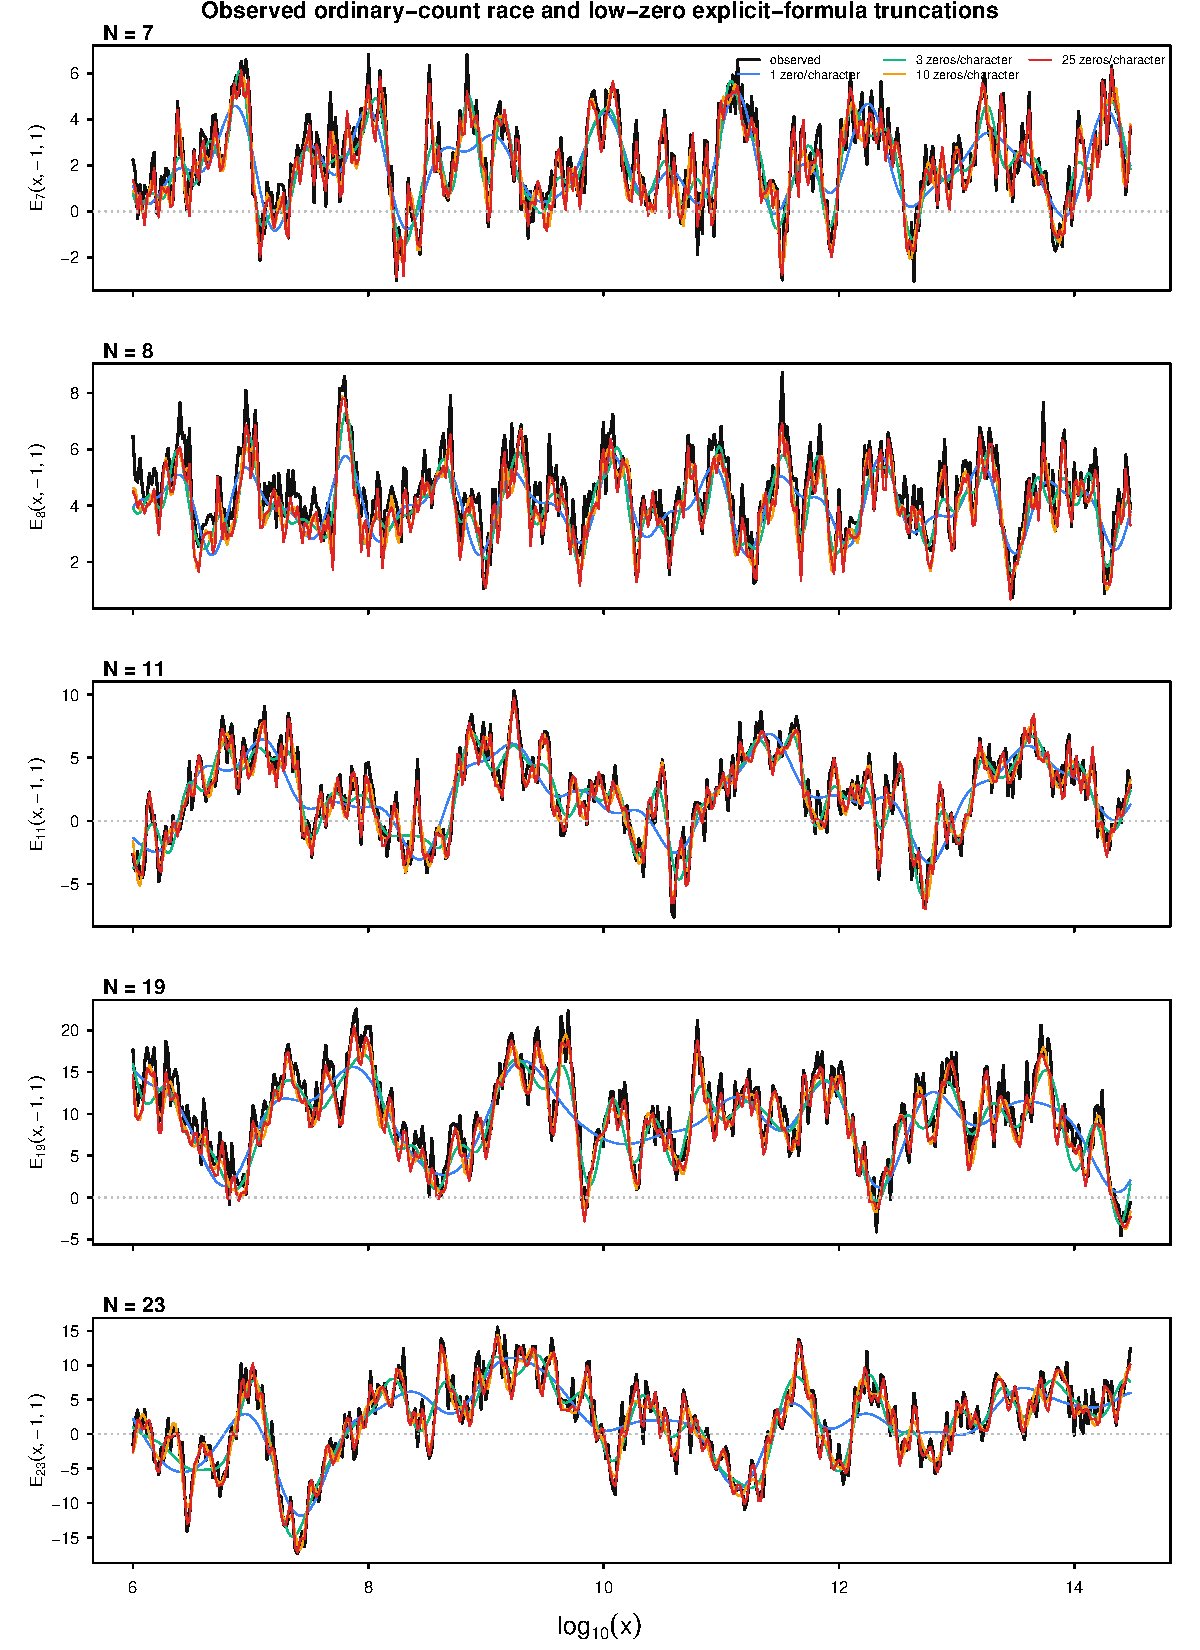
\includegraphics[width=\textwidth,height=0.82\textheight,keepaspectratio]{figures/spectral_reconstruction.pdf}
\caption{Observed normalized ordinary-count races (black) and
explicit-formula truncations using $K=1,3,10,25$ positive zeros per
nonprincipal character.  The panels show the class $a=-1\pmod N$.}
\label{fig:spectral-reconstruction}
\end{figure}

\subsection{The very low odd-character mode modulo 19}

For the primitive character of Conrey index 13 modulo 19, of order 18,
\begin{equation}\label{eq:n19-zero}
 \gamma=0.0189563990802261\ldots,\qquad \chi(-1)=-1.
\end{equation}
An independent Python FLINT/Arb computation gives opposite, sign-definite
Hardy-$Z$ endpoint balls across a bracket of width $5.94\times10^{-84}$ and a
midpoint $L$-value upper bound below $3.55\times10^{-85}$.  This certifies
existence of a critical-line zero in the bracket, but not uniqueness,
completeness, or GRH.  Its top-decade RMS contribution to the $-1$ race is
$6.719$, and its correlation with the centered observed curve is $0.728$.

Using 100 positive ordinates for every nonprincipal character modulo 19 raises
the $-1$ correlation from $0.9715$ at $K=25$ to $0.9925$ at $K=100$; the
reconstruction still has 14 rank changes and 7 leader changes.  Therefore the
previous $\gamma\approx1.74$ one-mode calculation and its
$e^{33.4}$ ``settling scale'' cannot be retained.  The data show a slow active
mode and do not identify $3\times10^{14}$ as a stabilization threshold.

The defensible finite-scale conclusion is that the ordinary races remain
spectrally coherent but dynamically unsettled through $3\times10^{14}$.
Low-zero truncations explain much of the observed motion; they do not prove an
eventual ordinary-count ordering.

\FloatBarrier
\section{Conditional examples}
\label{sec:conditional-examples}

The special-value combinations for small moduli are useful test cases for
Conjecture \ref{conj:regularized-target}, but they are not unconditional
rankings of prime counts.  For $N=3$ and $4$ the character groups contain one
nonprincipal real character, and the selector of Lemma \ref{lem:selector}
reduces the proposed value to the corresponding real logarithm.  For $N=8$
and $12$ several real characters contribute.  Any displayed ordering in these
cases is conditional on the two-parameter limit, the common normalization, and
the independently recomputed $B_N(a)$ values.  We therefore do not promote the
previous small-modulus tables to theorems in this revision.

\section{Open analytic obligations}
\label{sec:open-obligations}

A theorem-level regularized result requires: (i) an unambiguous definition of
the statistic on both the prime and spectral sides; (ii) a proved $T(x)$
regime; (iii) a summed off-diagonal estimate uniform over the prime powers up
to $x$; (iv) justified order interchanges; (v) separate control of prime powers,
conductor, gamma, and imprimitive factors; (vi) a specified logarithm branch
with a reality proof; and (vii) strict inequalities if a universal ordering is
claimed.  The earlier Fej\'er-kernel ``independent proof'' is omitted because
its claimed uniform prime-tail bound was not established.

\section{Reproducibility, formalization, and declarations}

\subsection{Data and code}

The authoritative ordinary-count file has SHA-256 digest
\begin{center}
\ttfamily\footnotesize
57957bdb3ce3243272c3d4b8e9ffe7dfb734b759f48b63becf7ae6f924e1caab.
\end{center}
The versioned computational package contains the zero generator,
reconstruction code, complete tabular outputs, transition ledger, figure
source, verifier, and SHA-256 manifests.  The extended $3\times10^{14}$ curve
is one run; the 567 shared baseline cells through $1.3\times10^{13}$ have an
independent comparison.  A permanent public archive identifier has not yet
been assigned and must be added before submission.

\subsection{Lean scope}

Lean 4 formalizes selected finite and algebraic components only.  These are
the corrected character-selector identity (including the inverse-class
witness modulo 7) and four finite statements about the leading
quadratic-nonresidue mean.  The checked files contain no \texttt{sorry} or
\texttt{admit}.  Lean does not formalize Conjecture
\ref{conj:regularized-target}, the explicit-formula estimates, the numerical
pipeline, DRH, or this manuscript as a whole.

\subsection{Author contributions}

Shin-ya Koyama initiated the regularized prime-bias framework and developed
its analytic formulation and intended number-theoretic applications.  Saar
Shai designed and performed the ordinary prime-count computations through
$3\times10^{14}$, checked the shared baseline, developed the low-zero spectral
reconstruction and verification pipeline, analyzed rank transitions and
individual modes, identified and independently certified the very low active
modulus-19 mode, formalized selected finite character-algebra and
quadratic-nonresidue statements in Lean 4, and wrote the numerical and
reproducibility sections.  Both authors are responsible for the interpretation,
the final mathematical claims, and approval of the submitted version.

\subsection{Computational and AI assistance}

Large-language-model tools assisted with manuscript revision, portions of the
computational workflow, code review, and proposals for selected Lean 4 proof
code.  The character-selector certificate returned through the Aristotle
interface was downloaded and recompiled against the stated Lean 4 and Mathlib
environment.  It does not certify the analytic results or the manuscript as a
whole.  Numerical claims were checked against versioned data, executable
verifiers, and artifact manifests.  The authors remain responsible for all
mathematical statements, computations, code, interpretations, and final text.

% =========================================================================
% References
% =========================================================================
\begin{thebibliography}{99}

\bibitem{AK23}
M.~Aoki and S.~Koyama,
\textit{ Chebyshev's bias against splitting and principal primes in global fields},
J. Number Theory \textbf{245} (2023), 233–262.

\bibitem{FM00}
A.~Feuerverger and G.~Martin,
\textit{Biases in the prime number race},
Experiment. Math. \textbf{9} (2000), no.~4, 535--570.

\bibitem{IK}
H.~Iwaniec and E.~Kowalski,
\textit{Analytic Number Theory},
American Mathematical Society Colloquium Publications, vol.~53, American Mathematical Society, Providence, RI, 2004.

\bibitem{RS94}
M.~Rubinstein and P.~Sarnak,
\textit{Chebyshev's bias},
Exp. Math. \textbf{2} (1994), no.~3, 173--197.

\end{thebibliography}
\end{document}
